\documentclass[letterpaper]{article}
\usepackage[margin=1in]{geometry}
\usepackage[utf8]{inputenc}
\usepackage{textcomp}
\usepackage{amssymb}
\usepackage{natbib}
\usepackage{graphicx}
\usepackage{gensymb}
\usepackage{amsthm, amsmath, mathtools}
\usepackage[dvipsnames]{xcolor}
\usepackage{enumerate}
\usepackage{mdframed}
\usepackage[most]{tcolorbox}
\usepackage{csquotes}
% https://tex.stackexchange.com/questions/13506/how-to-continue-the-framed-text-box-on-multiple-pages

\tcbuselibrary{theorems}

\newcommand{\R}{\mathbb{R}}
\newcommand{\Z}{\mathbb{Z}}
\newcommand{\N}{\mathbb{N}}
\newcommand{\Q}{\mathbb{Q}}
\newcommand{\C}{\mathbb{C}}
\newcommand{\code}[1]{\texttt{#1}}
\newcommand{\mdiamond}{$\diamondsuit$}
\newcommand{\PowerSet}{\mathcal{P}}
\newcommand{\Mod}[1]{\ (\mathrm{mod}\ #1)}
\DeclareMathOperator{\lcm}{lcm}

%\newtheorem*{theorem}{Theorem}
%\newtheorem*{definition}{Definition}
%\newtheorem*{corollary}{Corollary}
%\newtheorem*{lemma}{Lemma}
\newtheorem*{proposition}{Proposition}


\newtcbtheorem[number within=section]{theorem}{Theorem}
{colback=green!5,colframe=green!35!black,fonttitle=\bfseries}{th}

\newtcbtheorem[number within=section]{definition}{Definition}
{colback=blue!5,colframe=blue!35!black,fonttitle=\bfseries}{def}

\newtcbtheorem[number within=section]{corollary}{Corollary}
{colback=yellow!5,colframe=yellow!35!black,fonttitle=\bfseries}{cor}

\newtcbtheorem[number within=section]{lemma}{Lemma}
{colback=red!5,colframe=red!35!black,fonttitle=\bfseries}{lem}

\newtcbtheorem[number within=section]{example}{Example}
{colback=white!5,colframe=white!35!black,fonttitle=\bfseries}{def}

\newtcbtheorem[number within=section]{note}{Important Note}{
        enhanced,
        sharp corners,
        attach boxed title to top left={
            xshift=-1mm,
            yshift=-5mm,
            yshifttext=-1mm
        },
        top=1.5em,
        colback=white,
        colframe=black,
        fonttitle=\bfseries,
        boxed title style={
            sharp corners,
            size=small,
            colback=red!75!black,
            colframe=red!75!black,
        } 
    }{impnote}
\usepackage[utf8]{inputenc}
\usepackage[english]{babel}
\usepackage{fancyhdr}
\usepackage[hidelinks]{hyperref}

\pagestyle{fancy}
\fancyhf{}
\rhead{CSE 105}
\chead{Wednesday, January 19, 2022}
\lhead{Lecture 5}
\rfoot{\thepage}

\setlength{\parindent}{0pt}

\begin{document}

\section{Nondeterministic Finite Automata (1.2, Continued)}
This continues from the notes from Monday, January 12.

\subsection{Equivalence of NFAs and DFAs}
Deterministic and nondeterministic finite automata both recognize the same class of languages.

\begin{theorem}{}{}
    Every nondeterministic finite automaton has an equivalent deterministic finite automaton.
\end{theorem}
\textbf{Remark:} Here, we say that two machines are equivalent if they recognize the same language. 

\bigskip 

The proof is as follows\footnote{This proof was used in our submission for HW2 Problem 3 (CSE 105, WI22). The group members involved in this submission are (only initials and the last two digits of their PID are shown): CB (67), TT (96), ASRJ (73), and me.}:
\begin{mdframed}[]
    \begin{proof}
        Let $N = (Q, \Sigma, \delta, q_0, F)$ be the NFA that recognizes the language $L$. We want to show that there is a DFA $M = (Q', \Sigma, \delta', q_0', F')$ which recognizes the same $L$. 
        \begin{enumerate}
            \item First, $Q' = \mathcal{P}(Q)$. This is because must have the states in $Q'$ to represents the possible subset of states in $Q$. In an NFA, we can make multiple copies of the automaton, which may end up at different states over time. We therefore need to account for where these copies can be in our corresponding DFA. 
 
            \item The alphabet $\Sigma$ is the same in both the NFA and DFA. 
 
            \item The transition function of the corresponding DFA is defined by: 
            \[\delta'(X, x) = \{q \in Q \mid q \in \delta(r, x) \text{ for some } r \in X \text{ or accessible via } \epsilon \text{ transitions}\}\]
            Where $X$ is a state of the DFA and $x \in \Sigma$. Because a state in an NFA can have multiple outgoing transition arrows under the same type (e.g. two outgoing arrows for \texttt{a}), we need to account for this in the corresponding NFA. This is our first condition in our $\delta'$ function; in this sense, if we consider the possible states that we can go to in the NFA, then the corresponding state in our DFA is the union of all of those possible states. 
            We must also consider that, for a given state in an NFA, there may be $\epsilon$ transitions. In case there are $\epsilon$ transitions, we need to consider where the $\epsilon$ transitions put a copy of the machine.

            \item The start state in the corresponding DFA is the set $q_0' = \{q_0\} \cup \delta^{*} (q_0, \epsilon)$. First, we note that the start state in the NFA is $q_0$; thus, the start state in the corresponding DFA must be \emph{at least} $\{q_0\}$. However, if there are any $\epsilon$ transitions from the start state, we must consider those as well since transitioning to another state from the state state via the $\epsilon$ transition doesn't consume any input. 

            \item The set of final states in the corresponding DFA is simply:
            \[F' = \{X \mid X \subseteq Q \text{ and } X \cap F \neq \emptyset\}\]
            Here, we're saying that if there are any sets in $Q'$ which contain a final state in $F$, then said set must be a final set. This is because, in a NFA, we may have multiple copies of the machine running, and if one copy stops at a final state, then the NFA is accepted (despite the other copies not necessarily being at a final state).
        \end{enumerate}
        The rest of the proof is omitted for now. 
    \end{proof}
\end{mdframed}

\subsubsection{Example: NFA to DFA}
Consider the following NFA $N$:
\begin{center}
    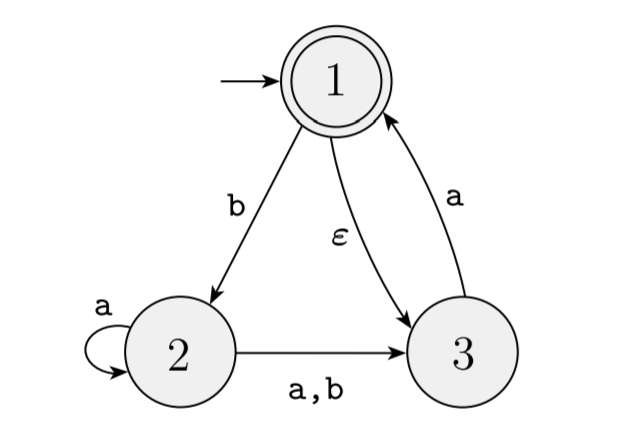
\includegraphics[scale=0.5]{../assets/nfa_to_dfa_1.png}

    \textbf{Figure:} The NFA $N$. 
\end{center}
We can define $N = (Q, \Sigma, \delta, q_0, F)$ like so: 
\begin{itemize}
    \item $Q = \{\code{1}, \code{2}, \code{3}\}$
    \item $\Sigma = \{\code{a}, \code{b}\}$
    \item $\delta$ is defined by 
    \begin{center}
        \begin{tabular}{c|c c c}
                & \code{a} & \code{b} & $\epsilon$ \\ 
            \hline 
            1   & $\emptyset$ & $\{2\}$ & $\{3\}$ \\ 
            2   & $\{2, 3\}$ & $\{3\}$ & $\emptyset$ \\ 
            3   & $\{1\}$ & $\emptyset$ & $\emptyset$
        \end{tabular}
    \end{center}
    \item $q_0 = 1$
    \item $F = \{1\}$
\end{itemize}
We're now being asked to construct a corresponding DFA: 
\[D = (Q', \Sigma', \delta', q_0', F')\]
Here, it's trivial to note that: 
\begin{itemize}
    \item $Q' = \PowerSet(Q) = \{\emptyset, \{1\}, \{2\}, \{3\}, \{1, 2\}, \{1, 3\}, \{2, 3\}, \{1, 2, 3\}\}$. 
    \item $\Sigma = \{\code{a}, \code{b}\}$
    \item $q_0 = \{1, 3\}$. This is because we can start at both state 1 and 3 since 3 has an $\epsilon$ transition.
    \item $F' = \{\{1\}, \{1, 2\}, \{1, 3\}, \{1, 2, 3\}\}$. This is because we want all subsets that contain $N$'s accept state. 
\end{itemize}
The hard part is actually ``wiring'' the DFA up, i.e. the transition function. To do this, we need to analyze how the NFA acts and ``translate'' it to what the DFA would do. So, let's consider each element in $Q'$ and see how it would relate to the NFA. 
\begin{itemize}
    \item Consider $\{1\} \in Q'$. In the NFA:
    \begin{itemize}
        \item $1$ doesn't go anywhere when \code{a} is given by itself. \textbf{However}, $1$ can go to $3$ since this is an $\epsilon$ transition, and $3$ goes to $1$ when consuming \code{a}, so it follows that $\boxed{\{1\} \xrightarrow{\code{a}} \{1, 3\}}$ in the corresponding DFA. 
        \item $1$ goes to $2$ when \code{b} is given, so it follows that $\boxed{\{1\} \xrightarrow[]{\code{b}} \{2\}}$ in the corresponding DFA. 
    \end{itemize}
    \item Consider $\{2\} \in Q'$. In the NFA: 
    \begin{itemize}
        \item $2$ goes to $2$ \emph{and} $3$ when \code{a} is given, so it follows that $\boxed{\{2\} \xrightarrow{\code{a}} \{2, 3\}}$ in the corresponding DFA. 
        \item $2$ goes to $3$ when \code{b} is given, so it follows that $\boxed{\{2\} \xrightarrow[]{\code{b}} \{3\}}$ in the corresponding DFA. 
    \end{itemize}
    \item Consider $\{3\} \in Q'$. In the NFA: 
    \begin{itemize}
        \item $3$ goes to $1$ when \code{a} is given, but then it can also go to $3$ since there is an $\epsilon$ transition, so it follows that $\boxed{\{3\} \xrightarrow{\code{a}} \{1, 3\}}$. 
        \item $3$ doesn't go anywhere when \code{b} is given, so it follows that $\boxed{\{3\} \xrightarrow{\code{b}} \emptyset}$.
    \end{itemize}
\end{itemize}
We can use the above to build cases for the remaining elements in $Q'$.
\begin{itemize}
    \item Consider $\{1, 2\} \in Q'$. In the corresponding NFA, this means that there's a copy at state $1$ and a copy at state $2$. So: 
    \begin{itemize}
        \item Suppose \code{a} is given. Then, from our previous work, we know that $\{1\} \xrightarrow{\code{a}} \{1, 3\}$, and $\{2\} \xrightarrow{\code{a}} \{2, 3\}$.
        Therefore, $\boxed{\{1, 2\} \xrightarrow{\code{a}} \{1, 2, 3\}}$ (recall that we take the union).
        \item Suppose \code{b} is given. Then, we know that $\{1\} \xrightarrow{\code{b}} \{2\}$, and $\{2\} \xrightarrow[]{\code{b}} \{3\}$. Therefore, $\boxed{\{1, 2\} \xrightarrow[]{\code{b}} \{2, 3\}}$. 
    \end{itemize}
    
    \item Consider $\{1, 3\} \in Q'$. In the corresponding NFA, this means that there's a copy at state $1$ and a copy at state $3$. So: 
    \begin{itemize}
        \item Suppose \code{a} is given. Then, from our previous work, we know that $\{1\} \xrightarrow{\code{a}} \{1, 3\}$, and $\{3\} \xrightarrow{\code{a}} \{1, 3\}$.
        Therefore, $\boxed{\{1, 3\} \xrightarrow{\code{a}} \{1, 3\}}$.
        \item Suppose \code{b} is given. Then, we know that $\{1\} \xrightarrow{\code{b}} \{2\}$, and $\{3\} \xrightarrow[]{\code{b}} \emptyset$. Therefore, $\boxed{\{1, 3\} \xrightarrow[]{\code{b}} \{2\}}$. 
    \end{itemize}
    
    \item Consider $\{2, 3\} \in Q'$. In the corresponding NFA, this means that there's a copy at state $2$ and a copy at state $3$. So: 
    \begin{itemize}
        \item Suppose \code{a} is given. Then, from our previous work, we know that $\{2\} \xrightarrow{\code{a}} \{2, 3\}$, and $\{3\} \xrightarrow{\code{a}} \{1, 3\}$.
        Therefore, $\boxed{\{2, 3\} \xrightarrow{\code{a}} \{1, 2, 3\}}$.
        \item Suppose \code{b} is given. Then, we know that $\{2\} \xrightarrow{\code{b}} \{3\}$, and $\{3\} \xrightarrow[]{\code{b}} \emptyset$. Therefore, $\boxed{\{2, 3\} \xrightarrow[]{\code{b}} \{3\}}$. 
    \end{itemize}

    \item Consider $\{1, 2, 3\} \in Q'$. In the corresponding NFA, this means that there's a copy at state $1$, $2$, and $3$. So: 
    \begin{itemize}
        \item Suppose \code{a} is given. From our previous work, we know that $\boxed{\{1, 2, 3\} \xrightarrow{\code{a}} \{1, 2, 3\}}$.
        \item Suppose \code{b} is given. From our previous work, we know that $\boxed{\{1, 2, 3\} \xrightarrow{\code{b}} \{2, 3\}}$.
    \end{itemize}
\end{itemize}

This gives us the following DFA: 
\begin{center}
    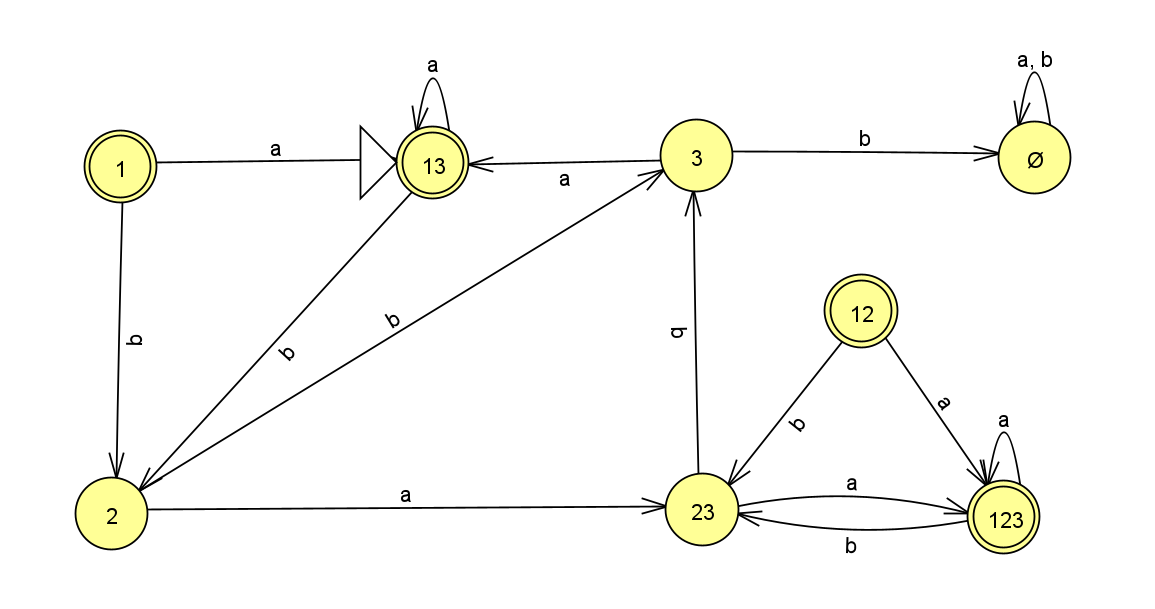
\includegraphics[scale=0.50]{../assets/nfa_to_dfa_2.png}
\end{center}

However, we note a few things.
\begin{itemize}
    \item State $1$ doesn't have anything coming into it. Therefore, we can remove it.
    \item State $12$ doesn't have anything coming into it. Therefore, we can remove it.
\end{itemize}
This gives us the simplified DFA: 
\begin{center}
    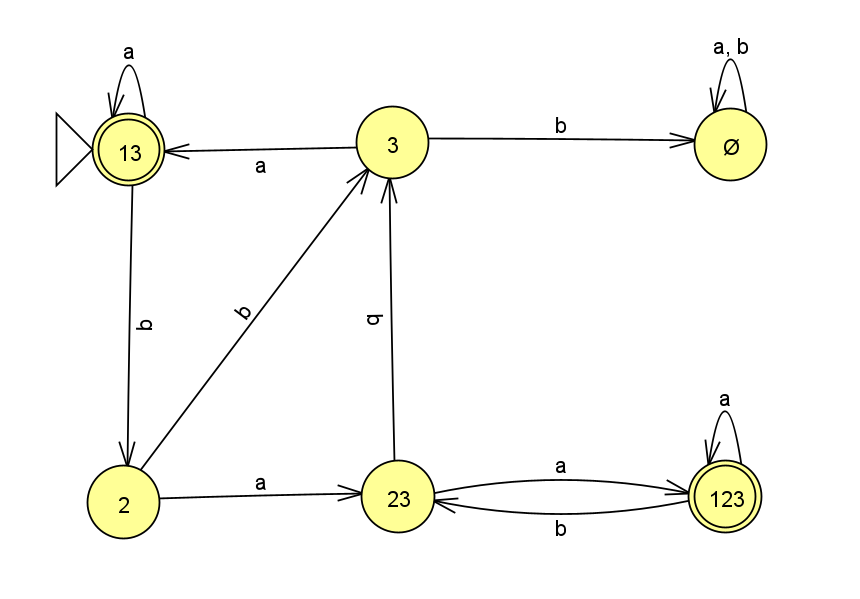
\includegraphics[scale=0.50]{../assets/nfa_to_dfa_3.png}
\end{center}

\subsection{Applications of Theorem}
There are several applications of this theorem. 

\begin{corollary}{}{}
    A language is regular if and only if some nondeterministic finite automaton recognizes it.
\end{corollary}


\begin{theorem}{}{}
    The class of regular languages is closed under the union operation.
\end{theorem}

\begin{mdframed}[]
    \begin{proof}
        (Sketch.) Suppose $A_1$ and $A_2$ are regular languages. We want to show that $A_1 \cup A_2$ is regular. We can take two NFAs, $N_1$ for $A_1$ and $N_2$ for $A_2$, and combine them to make one new NFA $N$. The idea is that $N$ must accept its input if either $N_1$ and $N_2$ accepts. So, essentially, we want to run both $N_1$ and $N_2$ in parallel. To simulate this behavior, we can create a new start state $q_0$ with two $\epsilon$ transitions pointing to the original start states of $N_1$ and $N_2$ (everything else about $N_1$ and $N_2$ are left unchanged).    
    \end{proof}
\end{mdframed}


\begin{theorem}{}{}
    The class of regular languages is closed under the concatenation operation.
\end{theorem}

\begin{mdframed}[]
    \begin{proof}
        (Sketch.) Suppose $A_1$ and $A_2$ are regular languages. We want to show that $A_1 \circ A_2$ is regular. We can take two NFAs, $N_1$ for $A_1$ and $N_2$ for $A_2$, and combine them to make one new NFA $N$. The idea for $N$ is as follows: 
        \begin{itemize}
            \item Start at the starting state for $N_1$ and remove the starting state for $N_2$. 
            \item Connect each accept state in $N_1$ to the original start state in $N_2$. The accept states in $N_1$ will no longer be accept states.  
        \end{itemize}
        By starting at the $N_1$ part of $N$, we guarantee that we will recognize some language $A_1$. Then, once we hit the original accept state in $N_1$, we can evaluate the rest of the string in $N_2$. If we hit an accept state in $N_2$, then we have recognized $A_1 \circ A_2$. 
    \end{proof}    
\end{mdframed}


\begin{theorem}{}{}
    The class of regular languages is closed under the union operation.
\end{theorem}

\begin{mdframed}[]
    \begin{proof}
        Suppose $A_1$ is a regular language. We want to show that $A_1^*$ is also regular. Consider the NFA $N_1$ for $A_1$. We want to modify $N_1$ so it recognizes $A_1^*$. Thus, our idea for the new NFA $N$ is as follows: 
        \begin{itemize}
            \item Because $\epsilon$ (the empty string) is valid under $A_1^*$, we must make a new start state that goes to the original start state; then, we can make the transition from the new start state to the original start state $\epsilon$. 
            \item We can connect the accept states in $N_1$ back to the original start state (not the new start state) with the labels being $\epsilon$.
            \item The accept states in $N_1$ is the same for $N$. 
        \end{itemize}
        By starting at the new start state, we can guarantee that $\epsilon$ will be accepted if it is the only thing to be read. Processing the string is as expected. However, once we reach the accept state, we need to \emph{go back} to the original start state to process the next ``word.'' This process keeps going until we no longer have any words to process. In this case, if we end off at any accept state with nothing left to read, then we accept. 
    \end{proof}
\end{mdframed}

\end{document}